\subsubsection{ClientController}
\begin{figure}[H]
	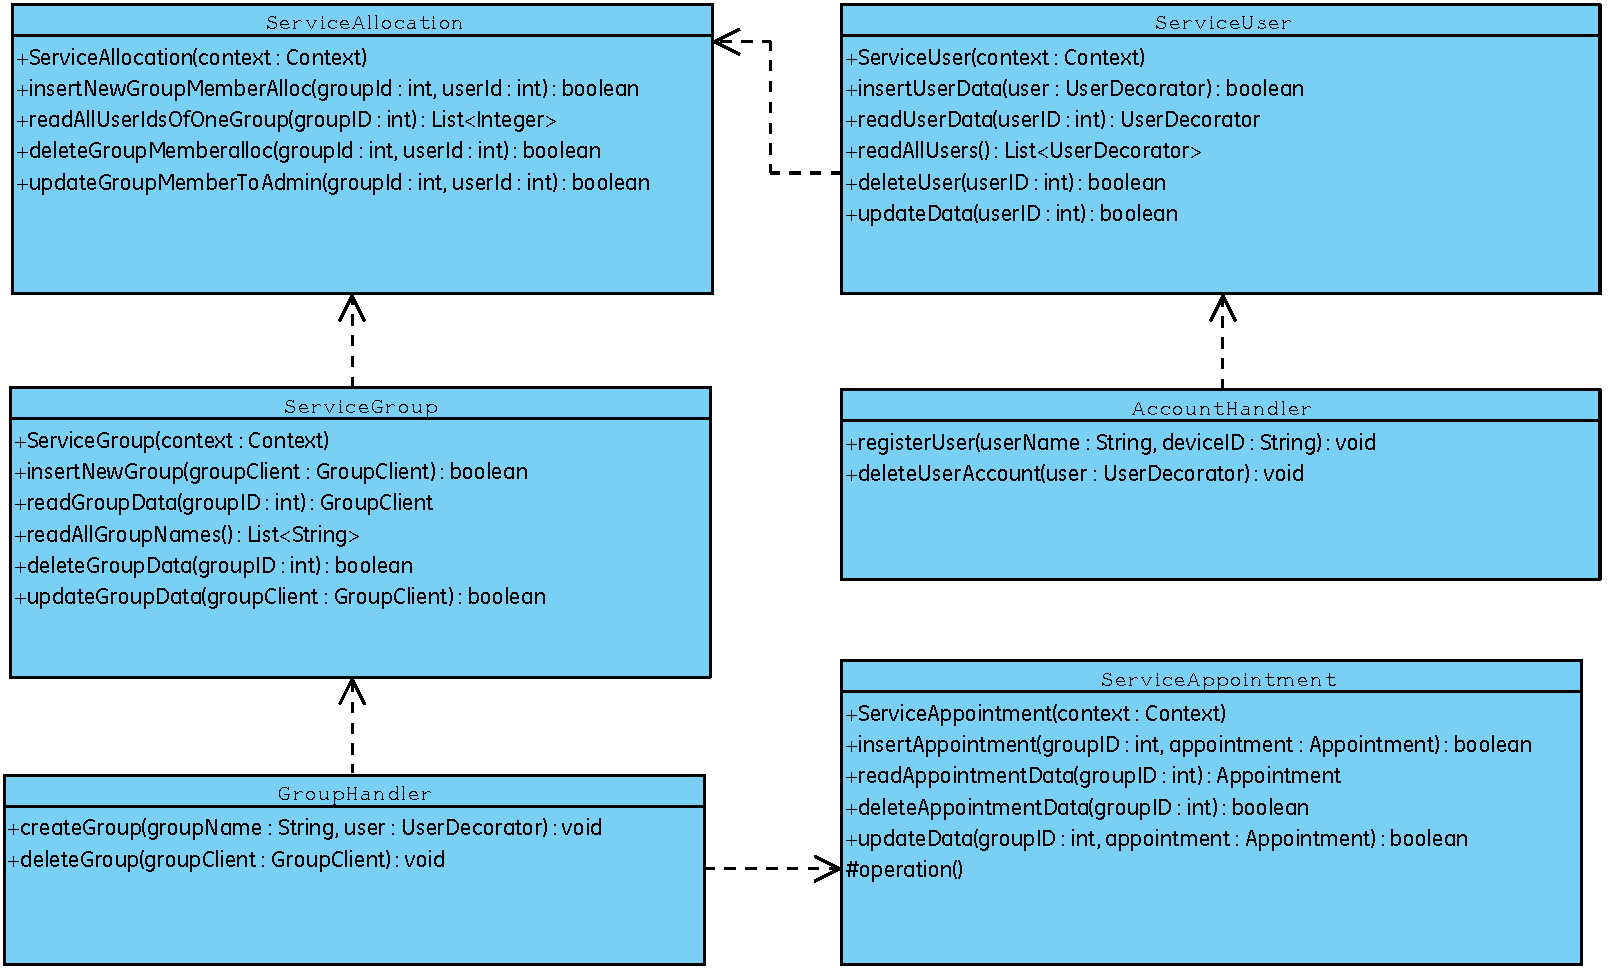
\includegraphics[scale = .5]{res/umlDiagramms/clientControllerDatabase.pdf}
	\centering
\end{figure}

\textbf{NetworkIntentService}

\paragraph{Database}

\textbf{Services}\\
Die folgenden Service Klassen stellen die grundlegenden Funktionen zur Verfügung, mit welchen auf die Daten der in den Innenklassen von FeedReaderContract definierten Tabellen der Datenbank zugegriffen werden kann. Dabei können Daten hinzugefügt (insert), gelesen (read), gelöscht (delete) und verändert (update) werden.
Weitere Details dazu, wie die jeweilige Datenbanken aufgebaut sind, finden sie in FeedEntryGroup, FeedEntryUser, FeedEntryAppointment, FeedEntryAllocation.

\begin{figure}[H]
	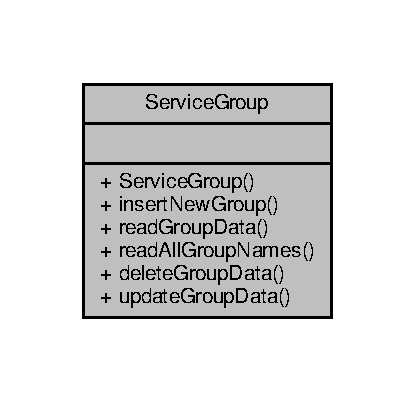
\includegraphics[scale = 1]{res/umlClasses/service_group__coll__graph.pdf}
	\centering
\end{figure}
In der Datenbank auf die ServiceGroup zugreift, werden die Gruppen gespeichert und ob der aktuelle Nutzer der Go-App für diese spezielle Gruppe seinen Go-Button aktiviert hat oder nicht. 
\begin{enumerate}
	\item public ServiceGroup(context: Context)\\
		Konstruktor, dem den Kontext der Applikation mitgegeben wird.
	\item public insertNewGroup(groupClient: GroupClient):boolean\\
		Eine neue Gruppe wird der Datenbank hinzugefügt und der GoStatus des Erstellers auf false gesetzt.
	\item public readGroupData(groupID: int):GroupClient \\
		Informationen über Gruppenname und GoStatus lesen. 
	\item public readAllGroupNames():List<String>\\
		Alle Gruppen in denen der aktuelle Benutzer Mitglied ist werden zurückgegeben.
	\item public deleteGroupData(groupID: int):boolean\\
		Eine Gruppe wird aus der Datenbank gelöscht.
	\item public updateGroupData(groupClient: GroupClient ):boolean\\
		Gruppendaten werden aktualisiert, wenn sich der Gruppenname oder der GoStatus ändert.
\end{enumerate}

\begin{figure}[H]
	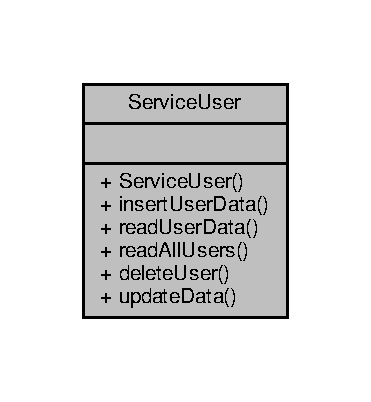
\includegraphics[scale = 1]{res/umlClasses/service_user__coll__graph.pdf}
	\centering
\end{figure}
In der Datenbank auf die ServiceUser zugreift ist der Name und die zuletzt bekannte Position des Benutzers gespeichert, welche bei neuen Informationen angepasst werden. 
\begin{enumerate}
	\item public ServiceUser(context: Context)\\
		Konstruktor, dem den Kontext der Applikation mitgegeben wird.
	\item public insertUserData(UserDecorator user):boolean\\
		Ein neuer Benutzer wird der Datenbank hinzugefügt, sobald dieser mit dem aktuellen Benutzer in einer Gruppe ist.
	\item public readUserData(userID: int):UserDecorator\\
		Inforamtionen über Benutzername und Position eines Benutzers können gelesen werden.
	\item public readAllUsers():List<UserDecorator> \\
		Alle Benutzernamen mit denen der aktuelle Benutzer in einer Gruppe ist lesen.
	\item public deleteUser(userID: int):boolean\\
		Einen Benutzer von der Datenbank entfernen.
	\item public updateData(userID: int):boolean\\
		Benutzerdaten anpassen, wenn sich Name oder Position geändert haben.
\end{enumerate}

\begin{figure}[H]
	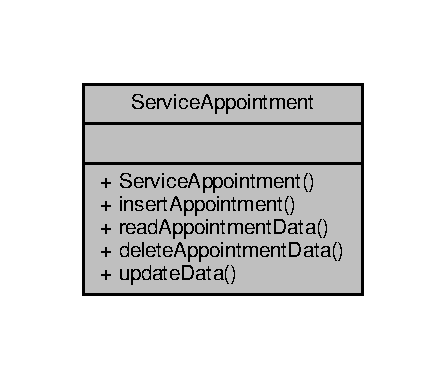
\includegraphics[scale = 1]{res/umlClasses/service_appointment__coll__graph.pdf}
	\centering
\end{figure}
In der Datenbank auf die ServiceAppointment zugreift, wird zu jeder Gruppe das aktuelle Treffen gespeichert und verändert, sobald ein neues existiert.
\begin{enumerate}
	\item public ServiceAppointment(context: Context)\\
		Konstruktor, dem den Kontext der Applikation mitgegeben wird.
	\item public insertAppointment(groupID: int, appointment: Appointment):boolean\\
		Wird aufgerufen wenn eine neue Gruppe erstellt wird. Dabei wird ein default Appointment initialisiert.
	\item public readAppointmentData(groupID: int):Appointment \\
		Informationen über Datum, Uhrzeit, Zielortname und Zielortposition können abgerufen werden.
	\item public deleteAppointmentData(groupID: int):boolean \\
		Wenn eine Gruppe gelöscht wird, wir auch das dazugehörige Appointment gelöscht.
	\item public updateData(groupID: int, appointment: Appointment):boolean \\
		Das Appointment wird angepasst, sobald es geändert wird.
\end{enumerate}

\begin{figure}[H]
	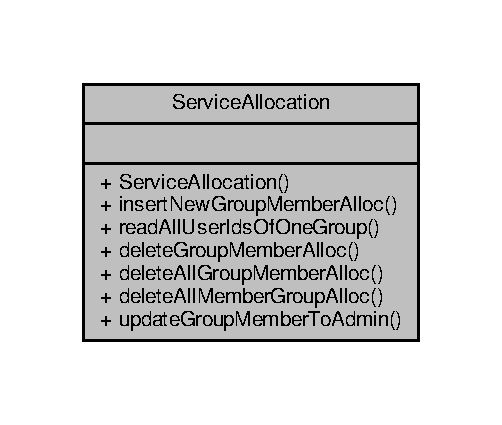
\includegraphics[scale = 1]{res/umlClasses/service_allocation__coll__graph.pdf} 
	\centering
\end{figure}
In der Datenbank auf die ServiceAllocation zugreift, wird die Verbindung zwischen Gruppen und Gruppenmitgliedern bzw. Administratoren gespeichert. 
\begin{enumerate}
	\item public (context: Context):ServiceAllocation\\
		Konstruktor, dem den Kontext der Applikation mitgegeben wird.
	\item public insertNewGroupMemberAlloc(groupID: int , userID: int):boolean\\
		Wenn ein neues Mitglied einer Gruppe hinzugefügt wird, dann wird diese Verbindung hier eingetragen.
	\item public readAllUserIdsOfOneGroup(groupID: int ):List<Integer> \\
		Um alle Mitglieder einer Gruppe zu bekommen, müssen dafür alle Benutzer Id's mit derselben Gruppen Id zurückgegeben werden.
	\item public deleteGroupMemberAlloc(groupid: int, userId: int):boolean \\
		Wird ein Gruppenmitglied aus einer Gruppe entfernt, so wird auch die Verbindung von diesem zur Gruppe gelöscht.
	\item public deleteAllGroupMemberAlloc(groupId: int):boolean \\
		Wird eine Gruppe gelöscht, so werden alle Verbindungen zu Benutzern dieser Gruppe gelöscht.
	\item public updateGroupMemberToAdmin(groupId: int , userID: int):boolean \\
		Wird ein Gruppenmitglied zum Administrator gemacht, dann wird dies in der Datenbank angepasst.
\end{enumerate}
	

\paragraph{ObjectStructure}

In Account- und GroupHandler werden allgemeine Funktionen definiert, die nicht selbst vom GroupClient oder von Unterklassen von UserComponent ausgeführt werden können, sondern eine übergeordnete Position benötigen.

\textbf{AccountHandler}
\begin{figure}[H]
	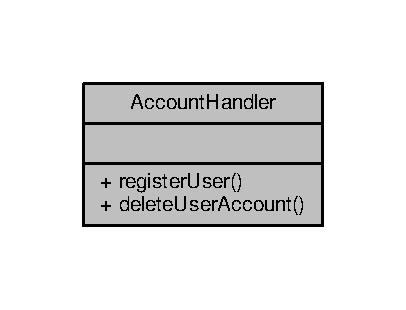
\includegraphics[scale = 1]{res/umlClasses/account_handler__coll__graph.pdf}
	\centering
\end{figure}
Die AccountHandler Klasse handelt das Registrieren und löschen vom aktuellen Benutzer ab.
\begin{enumerate}
	\item public registerUser(userName: String, deviceID: String)\\
		Ein neuer Benutzer registriert sich mit einem Namen und seiner Gerätenummer. Dieser wird zunächst als SimpleUser Objekt angelegt und mit der Gerätenummer auf dem Server gespeichert, um Missbrauch zu verhindern.
	\item public deleteUserAccount(user: UserDecorator)\\
		Löscht ein Benutzer seinen Account, wird er von der Datenbank gelöscht.
\end{enumerate}

\textbf{GroupHandler}
\begin{figure}[H]
	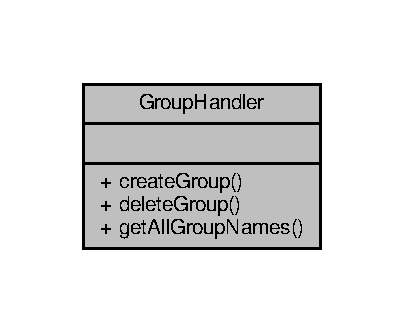
\includegraphics[scale = 1]{res/umlClasses/group_handler__coll__graph.pdf}
	\centering
\end{figure}
Die GroupHandler Klasse handelt das Erstellen und Löschen von Gruppen ab.
\begin{enumerate}
	\item public createGroup(groupName: String, user: UserDecorator)\\
		Eine neue Gruppe wird erstellt, mit einem eindeutigen Gruppennamen und mit dem Ersteller als Administrator.
	\item public deleteGroup(GroupClient groupClient)\\
		Eine Gruppe wird gelöscht und alle ihre Mitglieder entfernt.
\end{enumerate}

